\documentclass[11pt,letterpaper]{article}

\usepackage[margin=1in,headheight=14pt]{geometry}
\usepackage{amsmath,amssymb,amsthm,mathtools}
\usepackage{graphicx}
\usepackage{xcolor}
\usepackage{enumitem}
\usepackage{microtype}
\usepackage{fancyhdr}
\usepackage[colorlinks=true,linkcolor=blue,citecolor=blue,urlcolor=blue]{hyperref}

% Personal notation and theorem environments.
%!TEX root = EM_singular_models.tex

% PDF margin etc settings
%\setlength{\textwidth}{\paperwidth}
%\addtolength{\textwidth}{-6cm}
%\setlength{\textheight}{\paperheight}
%\addtolength{\textheight}{-4cm}
%\addtolength{\textheight}{-1.1\headheight}
%\addtolength{\textheight}{-\headsep}
%\addtolength{\textheight}{-\footskip}
%\setlength{\oddsidemargin}{0.5cm}
%\setlength{\evensidemargin}{0.5cm}

%%%%%%%%%%%%%%%%%%%%%%%%%%%%%%%%

% MACROS HERE

%%%%%%%%%%%%%%%%%%%%%%%%%%%%%%%%

\newcommand{\fixedpointtheta}{\widehat\theta_\obs}

\newcommand{\cover}{N}
\newcommand{\kinit}{\nu}
\newcommand{\cdelta}{c_\threshold}
\newcommand{\dndelta}{\omega}
\newcommand{\kndelta}{\Upsilon}
\newcommand{\kndeltanew}{\Psi}
\newcommand{\radii}{\mathcal{R}}
\newcommand{\event}{\mathcal{E}}
\newcommand{\kevent}{\mathcal{D}}


% Observations, dimension etc.
\newcommand{\dims}{\ensuremath{d}}
\newcommand{\samples}{\ensuremath{n}}
\newcommand{\obs}{\samples}
\newcommand{\real}{\ensuremath{\mathbb{R}}}
\newcommand{\complex}{\ensuremath{\mathbb{C}}}
\newcommand{\realdim}{\ensuremath{\real^\dims}}

\newcommand{\smallthreshold}{\epsilon}

% some mathcal notations
\newcommand{\order}[1]{\ensuremath{\mathcal{O}\parenth{#1}}}

% Basic statistics notation
\newcommand{\xstar}{\ensuremath{x^*}}
\newcommand{\xbar}{\ensuremath{\bar{x}}}
% True parameter
\newcommand{\thetastar}{\ensuremath{{\theta^*}}}
% Estimate one
\newcommand{\thetahat}{\ensuremath{\widehat{\theta}}}
% Estimate two
\newcommand{\thetatil}{\ensuremath{\widetilde{\theta}}}
\newcommand{\thetabar}{\ensuremath{\bar{\theta}}}
\newcommand{\yvec}{\ensuremath{y}}
\newcommand{\Xmat}{\ensuremath{X}}

% Distributions
\newcommand{\distribution}{P}
\newcommand{\density}{f}
\newcommand{\gaussiandensity}{\phi}
\newcommand{\NORMAL}{\ensuremath{\mathcal{N}}}
\newcommand{\BER}{\ensuremath{\mbox{Ber}}}

% Spaces
\newcommand{\Xspace}{\ensuremath{\mathcal{X}}}
\newcommand{\Yspace}{\ensuremath{\mathcal{Y}}}
\newcommand{\Zspace}{\ensuremath{\mathcal{Z}}}


% Brackets Size
\newcommand{\brackets}[1]{\left[ #1 \right]}
\newcommand{\parenth}[1]{\left( #1 \right)}
\newcommand{\bigparenth}[1]{\big( #1 \big)}
\newcommand{\biggparenth}[1]{\bigg( #1 \bigg)}
\newcommand{\braces}[1]{\left\{ #1 \right \}}
\newcommand{\abss}[1]{\left| #1 \right |}
\newcommand{\angles}[1]{\left\langle #1 \right \rangle}
\newcommand{\tp}{^\top}

% Generic vectors and scalars
\newcommand{\myvec}{u} % for generic vector
\newcommand{\myvectwo}{v} % for generic vector
\newcommand{\mymat}{B}
\newcommand{\set}{{A}}
\newcommand{\scalar}{\alpha}
\newcommand{\tvscalar}{\epsilon}
\newcommand{\tailboundscalar}{t}
\newcommand{\term}{U}
\newcommand{\myVarone}{\alpha_X}
\newcommand{\myVartwo}{\alpha_Y}
\newcommand{\myCovmat}{\Sigma}
\newcommand{\xcord}[1]{x^{(#1)}}
\newcommand{\xcordpop}[1]{X^{(#1)}}
\newcommand{\ycordpop}[1]{Y^{(#1)}}
\newcommand{\myVarthree}{\ensuremath{U}}
\newcommand{\myVarfour}{\ensuremath{V}}
\newcommand{\myfuntwo}{\ensuremath{g}}
\newcommand{\numsteps}{t}
\newcommand{\totalnumsteps}{T}
\newcommand{\seqalpha}[1]{\alpha_{#1}}
\newcommand{\seqnu}[1]{\nu^{(#1)}}
\newcommand{\imax}{\ell_\smallthreshold}
\newcommand{\basis}{e}
\newcommand{\radem}{\varepsilon}
\newcommand{\Tone}{T\ensuremath{_{0}}}
\newcommand{\Ttwo}{T\ensuremath{_{2}}}
\newcommand{\contractPar}[1]{\ensuremath{\gamma\parenth{#1}}}

\newcommand{\simiid}{\overset{\mathrm{i.i.d.}}{\sim}}
\newcommand{\eqd}{\overset{d}{=}}


% EM updates
\newcommand{\hidden}{Z}
\newcommand{\qfun}[2]{Q(#1\vert#2)}
\newcommand{\variable}{\theta}
\newcommand{\weights}{w}
\newcommand{\myfun}{q}
\newcommand{\gradf}{\nabla \myfun}
\newcommand{\hessf}{\nabla^2 \myfun}
\newcommand{\iter}{t}
\newcommand{\mupdate}{M}
\newcommand{\mupdategeneral}{\ensuremath{M^{GN}}}




% EM contractions
\newcommand{\contractgene}{\ensuremath{\gamma^{GN}}}
\newcommand{\updateMat}{\ensuremath{\Gamma_{\theta}}}
\newcommand{\mymatTheta}{\ensuremath{B_{\theta}}}
\newcommand{\sech}{\text{sech}}

% Nhat's macros 
\newcommand{\Rspace}{\ensuremath{\mathbb{R}}}
\newcommand{\Ecal}{\ensuremath{\mathcal{E}}}
\newcommand{\Ncal}{\ensuremath{\mathcal{N}}}
\newcommand{\gradient}{\ensuremath{\nabla}}
\newcommand{\smallweight}{\ensuremath{\epsilon^{sw}}}
\newcommand{\smallnorm}{\ensuremath{\rho^{sw}}}
\newcommand{\ball}{\ensuremath{\mathbb{B}}}
\newcommand{\sphere}{\ensuremath{\mathbb{S}}}

\newcommand{\diam}{\ensuremath{\text{diam}}}
\newcommand{\upper}{\ensuremath{\bar{C}}}
\newcommand{\sample}{\ensuremath{\xi}}
\newcommand{\weight}{\ensuremath{\pi}}
\newcommand{\contracasym}{\ensuremath{\rho}}
\newcommand{\Fishermatrix}{\ensuremath{\mathcal{I}}}
\newcommand{\barcontracasym}{\ensuremath{\bar{\rho}}}


\newcommand{\TrueDensity}{\ensuremath{f}}
\newcommand{\FitDensity}{\ensuremath{f}_{\theta}}
\newcommand{\FitDensityfree}{\ensuremath{f}_{\pi, \theta}}
\newcommand{\FitDensitygen}{\ensuremath{f}_{\pi, \theta_{1}, \theta_{2}}}
\newcommand{\FitDensitymore}{\ensuremath{f}_{G}}
\newcommand{\normden}{\ensuremath{\phi}}
\newcommand{\mean}{\ensuremath{\theta}}
\newcommand{\sd}{\ensuremath{\sigma}}
\newcommand{\parFOS}{\ensuremath{\gamma}}
\newcommand{\funQ}{\ensuremath{Q}}
\newcommand{\updateM}{\ensuremath{M}}
\newcommand{\weightFun}{\ensuremath{w}}
\newcommand{\mydefn}{\ensuremath{:=}}
\newcommand{\poincare}{\ensuremath{\tilde{C}}}
\newcommand{\paraspace}{\ensuremath{\Theta}}
\newcommand{\loglihood}{\ensuremath{F}}
\newcommand{\prior}{\ensuremath{\pi}}
\newcommand{\posterior}{\ensuremath{\Pi}}
\newcommand{\boundcons}{\ensuremath{B}}
\newcommand{\boundconstot}{\ensuremath{H}}
\newcommand{\noise}{\ensuremath{\varepsilon}}
\newcommand{\loglihoodgaus}{\ensuremath{F^{G}}}
\newcommand{\loglihoodind}{\ensuremath{F^{I}}}
\newcommand{\loglihoodlogit}{\ensuremath{F^{R}}}
\newcommand{\noiseone}{\ensuremath{\varepsilon_{1}}}
\newcommand{\noisetwo}{\ensuremath{\varepsilon_{2}}}

%%%SDE_Bayesian_inf
\newcommand{\weakcon}{\ensuremath{\psi}}
\newcommand{\perturb}{\ensuremath{\zeta}}
\newcommand{\inver}{\ensuremath{\xi}}

% Universal constants
\newcommand{\unicon}{c}
\newcommand{\uniconnew}{c'}
\newcommand{\uniconone}{c_1}
\newcommand{\unicontwo}{c_2}

% some parameters that you may define
\newcommand{\scparam}{m} % strong  convexity parameter
\newcommand{\smoothness}{L} % smoothness parameter
\newcommand{\step}{h}


%%%%%%%%% Distributions and Random variables %%%%%%%%%%%
\newcommand{\rvg}{\xi} % to denote the random variable g
\newcommand{\threshold}{\delta}


%%%%%%%%% Basic Terms like defn, etal, tmix, polylog %%%%%%%%%%%
\newcommand{\defn}{:=}
\newcommand{\rdefn}{=:}
\newcommand{\etal}{{et al.}}
\newcommand{\polylog}{\text{poly-log}}

% Some vector/matrix norms
\newcommand{\matnorm}[3]{|\!|\!| #1 | \! | \!|_{{#2}, {#3}}}
\newcommand{\matsnorm}[2]{|\!|\!| #1 | \! | \!|_{{#2}}}
\newcommand{\vecnorm}[2]{\left\| #1\right\|_{#2}}
\newcommand{\enorm}[1]{\vecnorm{#1}{2}} % euclidean norm
\newcommand{\nucnorm}[1]{\ensuremath{\matsnorm{#1}{\footnotesize{\mbox{nuc}}}}}
\newcommand{\fronorm}[1]{\ensuremath{\matsnorm{#1}{\footnotesize{\mbox{fro}}}}}
\newcommand{\opnorm}[1]{\ensuremath{\matsnorm{#1}{\tiny{\mbox{op}}}}}
%%% EM paper
\newcommand{\constrainnorm}[1]{\vecnorm{#1}{[k]}} % euclidean norm

\newcommand{\bigmatsnorm}[2]{{\Big|\!\Big|\!\Big| #1
  \Big|\!\Big|\!\Big|}_{#2}}

% Inner product
\newcommand{\inprod}[2]{\ensuremath{\langle #1 , \, #2 \rangle}}

% Kullback-Leibler
\newcommand{\kull}[2]{\ensuremath{D_{\text{KL}}(#1\; \| \; #2)}}

% Probability
\newcommand{\Exs}{\ensuremath{{\mathbb{E}}}}
\newcommand{\Prob}{\ensuremath{{\mathbb{P}}}}

%Eigenvector / eigenvalue related notation
\newcommand{\eig}[1]{\ensuremath{\lambda_{#1}}}
\newcommand{\eigmax}{\ensuremath{\eig{\max}}}
\newcommand{\eigmin}{\ensuremath{\eig{\min}}}

% \DeclareMathOperator{\det}{det}
\DeclareMathOperator{\modd}{mod}
\DeclareMathOperator{\diag}{diag}
\DeclareMathOperator{\var}{var}
\DeclareMathOperator{\cov}{cov}
\DeclareMathOperator{\trace}{trace}
\DeclareMathOperator{\abs}{abs}
\DeclareMathOperator{\floor}{floor}
\DeclareMathOperator{\vol}{vol}
\DeclareMathOperator{\child}{child}
\DeclareMathOperator{\parent}{parent}
\DeclareMathOperator{\sign}{sign}
\DeclareMathOperator{\rank}{rank}
\DeclareMathOperator{\toeplitz}{toeplitz}




\newtheoremstyle{named}{}{}{\itshape}{}{\bfseries}{.}{.5em}{\thmnote{#3's }#1}
\theoremstyle{named}
\newtheorem*{namedtheorem}{Lemma}

%%%%%%%
\theoremstyle{plain}

% {Theorem, Proposition, Lemma, Corollary} numbered sequentially
% throughout the paper
\newtheorem{theorem}{Theorem}
\newtheorem{proposition}{Proposition}
\newtheorem{lemma}{Lemma}
\newtheorem{claim}{Claim}
\newtheorem{corollary}{Corollary}
\newtheorem{definition}{Definition}
\newtheorem{conjecture}{Conjecture}
\newtheorem{remark}{Remark}
%%%%%%%%%%%%%%%%%%%%%%%%%%%%%%%%%%%%%%%%%%%%%%%%%%%%%%%%%%%%%%%%%%%%%%%
% WIDEBAR COMMAND
\newlength{\widebarargwidth}
\newlength{\widebarargheight}
\newlength{\widebarargdepth}
\DeclareRobustCommand{\widebar}[1]{%
  \settowidth{\widebarargwidth}{\ensuremath{#1}}%
  \settoheight{\widebarargheight}{\ensuremath{#1}}%
  \settodepth{\widebarargdepth}{\ensuremath{#1}}%
  \addtolength{\widebarargwidth}{-0.3\widebarargheight}%
  \addtolength{\widebarargwidth}{-0.3\widebarargdepth}%
  \makebox[0pt][l]{\hspace{0.3\widebarargheight}%
    \hspace{0.3\widebarargdepth}%
    \addtolength{\widebarargheight}{0.3ex}%
    \rule[\widebarargheight]{0.95\widebarargwidth}{0.1ex}}%
  {#1}}



%%% New version of \caption puts things in smaller type, single-spaced
%%% and indents them to set them off more from the text.
\makeatletter
\long\def\@makecaption#1#2{
        \vskip 0.8ex
        \setbox\@tempboxa\hbox{\small {\bf #1:} #2}
        \parindent 1.5em  %% How can we use the global value of this???
        \dimen0=\hsize
        \advance\dimen0 by -3em
        \ifdim \wd\@tempboxa >\dimen0
                \hbox to \hsize{
                        \parindent 0em
                        \hfil
                        \parbox{\dimen0}{\def\baselinestretch{0.96}\small
                                {\bf #1.} #2
                                %%\unhbox\@tempboxa
                                }
                        \hfil}
        \else \hbox to \hsize{\hfil \box\@tempboxa \hfil}
        \fi
        }
\makeatother



%% COMMENTING commands

\long\def\comment#1{}
\definecolor{battleshipgrey}{rgb}{0.52, 0.52, 0.51}
\definecolor{darkgray}{rgb}{0.66, 0.66, 0.66}
\definecolor{darkgreen}{rgb}{0.0, 0.2, 0.13}
\definecolor{darkspringgreen}{rgb}{0.09, 0.45, 0.27}
\definecolor{dukeblue}{rgb}{0.0, 0.0, 0.61}
\definecolor{olivedrab7}{rgb}{0.24, 0.2, 0.12}
\definecolor{darkblue}{rgb}{0.0, 0.0, 0.55}
\definecolor{darkscarlet}{rgb}{0.34, 0.01, 0.1}
\definecolor{candyapplered}{rgb}{1.0, 0.03, 0.0}
\definecolor{ao(english)}{rgb}{0.0, 0.5, 0.0}
\definecolor{applegreen}{rgb}{0.55, 0.71, 0.0}

\newcommand{\red}[1]{\textcolor{red}{#1}}
\newcommand{\mjwcomment}[1]{{\bf{{\red{{MJW --- #1}}}}}}
\newcommand{\mwlcomment}[1]{{\bf{{\color{orange}{{Wenlong --- #1}}}}}}

\newcommand{\blue}[1]{\textcolor{blue}{#1}}
\newcommand{\green}[1]{\textcolor{green}{#1}}
\newcommand{\highlight}[1]{\textcolor{applegreen}{#1}}

% comment lines
\newcommand{\genecomment}[1]{{\bf{{\blue{{TEAM --- #1}}}}}}
\newcommand{\rrdcomment}[1]{{\bf{{\blue{{RRD --- #1}}}}}}
\newcommand{\nhcomment}[1]{{\bf{{\blue{{NH --- #1}}}}}}
\newcommand{\kkcomment}[1]{{\bf{{\darkgreen{{KK --- #1}}}}}}


\newcommand{\widgraph}[2]{\includegraphics[keepaspectratio,width=#1]{#2}}


\newcommand{\coursenumber}{STA3000F}
\newcommand{\coursetitle}{Advanced Theory of Statistics}
\newcommand{\courseterm}{Fall 2026}
\newcounter{lecture}
\setcounter{lecture}{4}
\newcommand{\lecturenumber}{\arabic{lecture}}
\newcommand{\lecturedate}{October 2, 2026}
\newcommand{\lecturer}{Wenlong Mou}

\pagestyle{fancy}
\fancyhf{}
\fancyhead[L]{\coursenumber: \coursetitle}
\fancyhead[R]{Lecture \lecturenumber}
\fancyfoot[C]{\lecturenumber--\arabic{page}}
\renewcommand{\headrulewidth}{0.4pt}
\renewcommand{\footrulewidth}{0pt}

\usepackage{bm}

\renewcommand{\thepage}{\lecturenumber--\arabic{page}}

\newtheorem{example}{Example}
\numberwithin{theorem}{lecture}
\numberwithin{proposition}{lecture}
\numberwithin{lemma}{lecture}
\numberwithin{claim}{lecture}
\numberwithin{corollary}{lecture}
\numberwithin{definition}{lecture}
\numberwithin{conjecture}{lecture}
\numberwithin{remark}{lecture}
\numberwithin{example}{lecture}
\numberwithin{equation}{lecture}
\counterwithin*{section}{lecture}
\renewcommand{\theHsection}{\arabic{lecture}.\arabic{section}}

\newcommand{\makelecturenotesheader}{%
  \noindent
  \textbf{\coursenumber: \coursetitle}%
  \hfill
  \textbf{\courseterm}

  \begin{center}
    {\Large\bfseries Lecture \lecturenumber: \lecturedate}
  \end{center}

  \noindent
  \textbf{Lecturer:} \lecturer
  \par\medskip
  \hrule
  \bigskip
}

\begin{document}

\makelecturenotesheader

\section{From Bayesian Cram\'{e}r--Rao to local minimax}
Idea: construct a prior distribution $\pi$ that is supported on a small neighborhood of $\theta_0$, and then use the inequality
\begin{align*}
  \sup_{|\theta - \theta_0| \leq r} \Exs_\theta \big[ |\widehat{\theta}_n - \theta|^2 \big] \geq \int_{|\theta - \theta_0| \leq r} \Exs_\theta \big[ |\widehat{\theta}_n - \theta|^2 \big] \pi (\theta) d\theta = r_\pi (\widehat{\theta}_n),
\end{align*}
for any possible estimator $\widehat{\theta}_n$.

Requirements for the prior $\pi$:
\begin{itemize}
  \item $\pi$ is supported on a small neighborhood of $\theta_0$.
  \item $\pi$ is smooth and vanishes on the boundary of its support.
  \item $\pi$ has small Fisher information $J(\pi)$.
\end{itemize}
Concrete choice:

Starting from the building block
\begin{align*}
  \nu_0 (x) = \cos^2 (\pi x / 2) \bm{1}_{x \in [-1, 1]}.
\end{align*}
For fixed radius $r > 0$, we define the prior
\begin{align*}
  \nu (\theta) = \frac{1}{r} \nu_0 ( (\theta - \theta_0) / r),
\end{align*}
which is supported on $[\theta_0 - r, \theta_0 + r]$.

The following illustration shows the shape and support of this local prior.
\begin{center}
  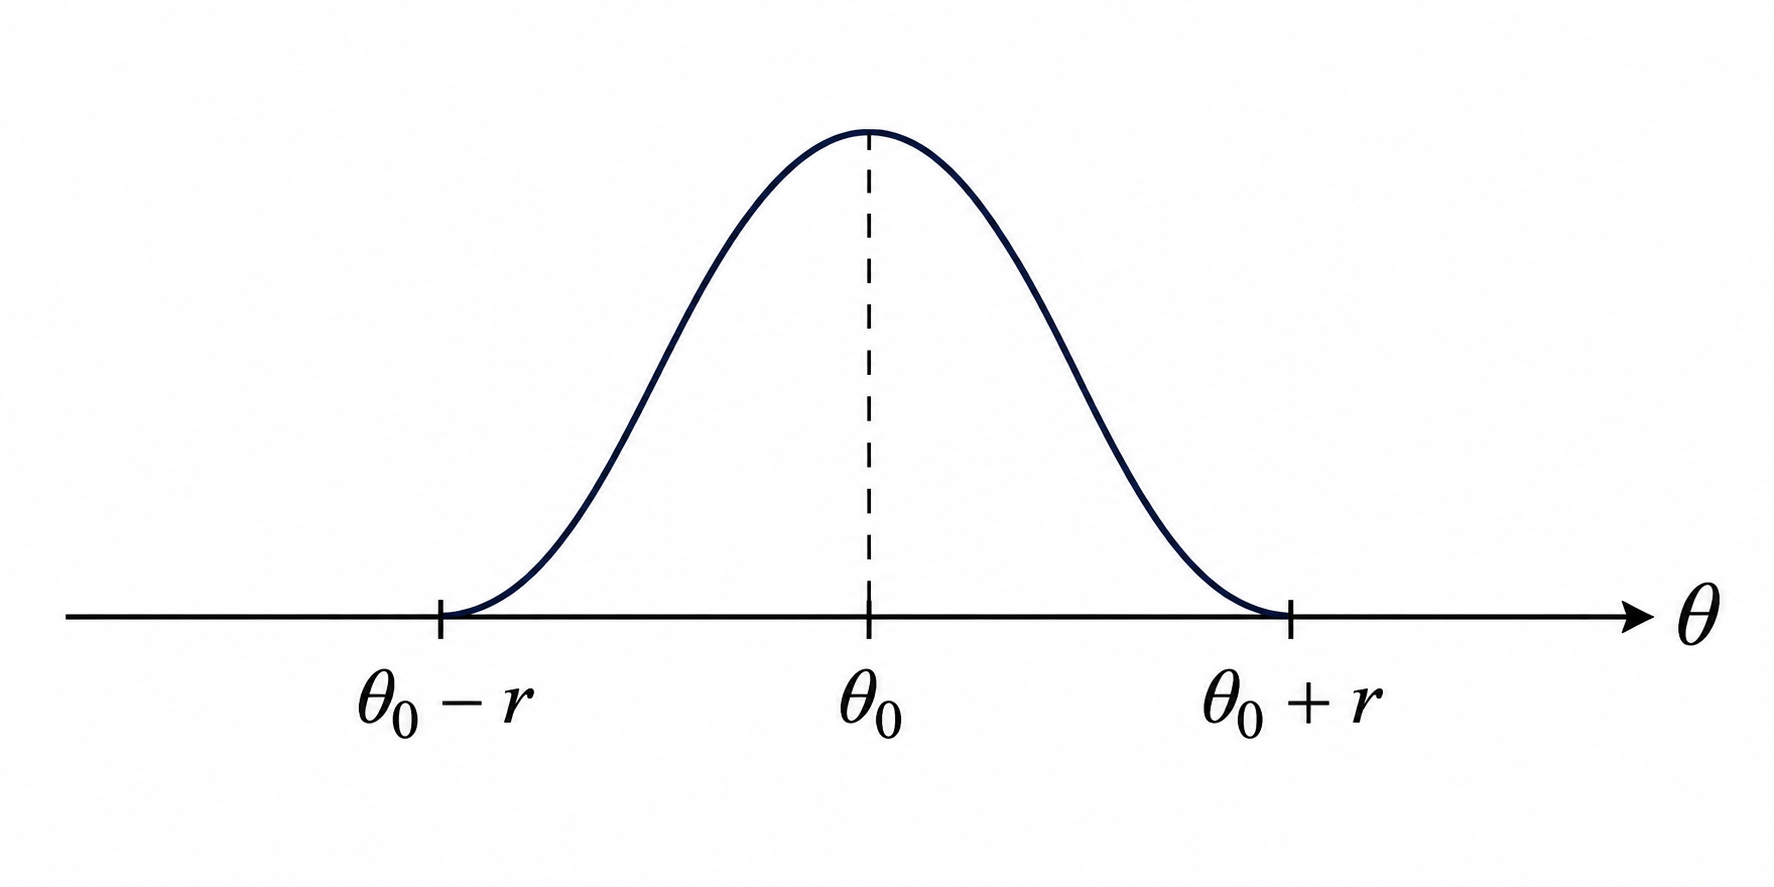
\includegraphics[width=0.75\textwidth]{./lec4-local-prior-illustration.png}

  \small The prior $\nu$ is centered at $\theta_0$ and vanishes at the endpoints $\theta_0-r$ and $\theta_0+r$. The dashed line marks its center.
\end{center}

Then we can compute the Fisher information of $\nu$ as
\begin{align*}
  J(\nu) = \int_{-1}^1 \frac{(\nu_0' (x))^2}{\nu_0 (x)} dx \cdot \frac{1}{r^2} = \frac{\pi^2}{r^2}.
\end{align*}
By putting them together, we arrive at a local minimax theorem
\begin{theorem}\label{thm:local-minimax-lower-bound}
  Under the same regularity conditions as the Bayesian Cram\'{e}r--Rao lower bound, given $n$ i.i.d. data, we have
  \begin{align*}
    \inf_{\widehat{\theta}_n} \sup_{|\theta - \theta_0| \leq r} \Exs_\theta \big[ |\widehat{\theta}_n - \theta|^2 \big] \geq \Big( n \int I (\theta) \nu (\theta) d \theta + \frac{\pi^2}{r^2} \Big)^{-1}.
  \end{align*}
\end{theorem}
When $r$ is small, the Fisher information $I(\theta)$ is approximately constant in the neighborhood of $\theta_0$. Furthermore, when $n$ is large, the term $\pi^2 / r^2$ is negligible. In that case, the lower bound is approximately $1 / (n I(\theta_0))$. But this does not require unbiasedness, and it is a local minimax lower bound. So this is a very general result.


Theorem~\ref{thm:local-minimax-lower-bound} is completely non-asymptotic. By taking the asymptotic regime where $n \rightarrow \infty$ and $r \rightarrow 0$, we can recover the classical asymptotic minimax lower bound
\begin{corollary}\label{cor:lam}
Under conditions of Theorem~\ref{thm:local-minimax-lower-bound}, we have
\begin{align*}
  \lim_{c \rightarrow + \infty} ~\lim\inf_{n \rightarrow + \infty}~ \inf_{\widehat{\theta}_n} ~\sup_{|\theta - \theta_0| \leq c / \sqrt{n}} n \cdot \Exs_\theta \big[ |\widehat{\theta}_n - \theta|^2 \big] \geq \frac{1}{I(\theta_0)}.
\end{align*}
\end{corollary}
Remarks:
\begin{itemize}
  \item The order of the limit is important. Here we consider a sequence of shrinking neighborhoods of $\theta_0$ as $n \rightarrow + \infty$, and $c$ controls the size relative to the parametric rate of $1/\sqrt{n}$. If you swap the order, you will get global minimax rate instead, which is typically much larger than the local minimax rate.
  \item The general local asymptotic minimax (LAM) theory is more general than the above corollary.
  \begin{enumerate}
    \item It requires less regularity conditions than the classical Cram\'{e}r--Rao lower bound (differentiability in quadratic mean, even weaker than first-order differentiability).
    \item General LAM theory works for general loss functions, not just squared error loss. For symmetric, bowl-shaped loss function $\ell$, we have
    \begin{align*}
      \lim_{c \rightarrow + \infty} ~\lim\inf_{n \rightarrow + \infty}~ \inf_{\widehat{\theta}_n} ~\sup_{|\theta - \theta_0| \leq c / \sqrt{n}} \Exs_\theta \big[ \ell \big( \sqrt{n} (\widehat{\theta}_n - \theta) \big) \big] \geq \Exs \big[ \ell (Z / \sqrt{I(\theta_0)}) \big], \quad Z \sim \mathcal{N} (0, 1).
    \end{align*}
  \end{enumerate}
  \item Under certain regularity conditions, the maximum likelihood estimator
  \begin{align*}
    \widehat{\theta}_n^{\mathrm{MLE}} \mydefn \arg\max_{\theta \in \Theta} \sum_{i=1}^n \log p_\theta (X_i)
  \end{align*}
  is known to satisfy the asymptotic convergence
  \begin{align*}
    \sqrt{n} (\widehat{\theta}_n^{\mathrm{MLE}} - \theta) \overset{d}{\longrightarrow} \mathcal{N} (0, I(\theta)^{-1}),
  \end{align*}
  So for a broad class of problems, MLE is asymptotically optimal in the sense of LAM theory.
  \item This easily extends to multivariate $\theta \in \real^d$.
\end{itemize}

\section{Hypothesis testing: a decision-theoretic perspective}
Basic framework:
\begin{align*}
  \text{Null hypothesis: } H_0: \theta \in \Theta_0, \quad \text{Alternative hypothesis: } H_1: \theta \in \Theta_1.
\end{align*}
Here $\Theta_0, \Theta_1 \subseteq \Theta$, and $\Theta_0 \cap \Theta_1 = \emptyset$. Testing is about making binary (or in general, discrete) decisions about where $\theta$ lies.

This is a decision-theoretic problem. The decision rule is the critical function (``the test'')
\begin{align*}
  \phi (x) = \begin{cases}
    1, & \text{reject } H_0,\\
    \pi \in (0, 1), & \text{randomized decision with probability } \pi,\\
    0, & \text{fail to reject } H_0.
  \end{cases}
\end{align*}
For estimation we don't usually use randomization (c.f. Rao--Blackwellization), but for testing, randomization is sometimes necessary to get optimal tests.

\begin{itemize}
  \item Significance level $\alpha$: we want to make sure that
  \begin{align*}
    \alpha_\phi \mydefn \sup_{\theta \in \Theta_0} \Exs_\theta [\phi (X)] \leq \alpha.
  \end{align*}
  \item Power function
  \begin{align*}
    \beta_\phi (\theta) \mydefn \Exs_{\theta} [\phi (X)], \quad \theta \in \Theta_1.
  \end{align*}
\end{itemize}
The role of two types of errors is asymmetric. Testing can be viewed as transforming multi-objective optimization into constrained optimization: we want to maximize the power function $\beta_\phi (\theta)$ for $\theta \in \Theta_1$, subject to the constraint that the significance level $\alpha_\phi$ is below a threshold $\alpha$.

Most desirable case:
\begin{definition}[Uniformly most powerful (UMP) test]
  A test $\phi^*$ is called uniformly most powerful (UMP) at level $\alpha$ if it satisfies the following conditions:
  \begin{enumerate}
    \item $\phi^*$ has significance level $\alpha$.
    \item For any other test $\phi$ with significance level $\alpha$, we have
    \begin{align*}
      \beta_{\phi^*} (\theta) \geq \beta_\phi (\theta), \quad \forall \theta \in \Theta_1.
    \end{align*}
  \end{enumerate}
\end{definition}
Of course, this is not always achievable. But in some special cases, we can construct UMP tests.
If this is not achievable, we can consider more restricted classes of tests, or to consider minimax optimality.

\subsection{Simple vs. simple testing}
\begin{align*}
  \Theta_0 = \{\theta_0\}, \quad \Theta_1 = \{\theta_1\}.
\end{align*}
Likelihood ratio test (LRT):
\begin{itemize}
\item Likelihood ratio statistic
\begin{align*}
  L (x) = \frac{p_{\theta_1} (x)}{p_{\theta_0} (x)}.
\end{align*}
\item LRT rejects when $L (x)$ is large. The critical function is
\begin{align*}
  \phi (x) = \begin{cases}
    1, & L (x) > c,\\
    \pi, & L (x) = c,\\
    0, & L (x) < c.
  \end{cases}
\end{align*}
We can choose $(c, \pi)$ to satisfy the significance level $\alpha$
\begin{align*}
  \Exs_{\theta_0} [\phi (X)] = \alpha.
\end{align*}
\end{itemize}
\begin{lemma}[Neyman--Pearson lemma]
  Given $\alpha \in (0, 1)$, the LRT $\phi^*_\alpha$ with significance level $\alpha$ exists, and it is the UMP test at level $\alpha$ for testing $H_0: \theta = \theta_0$ vs. $H_1: \theta = \theta_1$.
\end{lemma}
Proof idea:
We first show existence of the LRT with significance level $\alpha$.
\begin{itemize}
  \item When $(c =0, \pi = 1)$, we have $\Exs_{\theta_0} [\phi (X)] = 1 > \alpha$.
  \item When $(c \rightarrow + \infty, \pi = 0)$, we have
  \begin{align*}
    \alpha_\phi = \int p_0 (x) \bm{1}_{p_1 (x) / p_0 (x) > c} d\lambda(x) \leq \int p_0 (x) \frac{p_1 (x)}{c p_0 (x)} d\lambda(x) = \frac{1}{c} \rightarrow 0 < \alpha.
  \end{align*}
\end{itemize}
We increase $c$ from $0$ to $+\infty$, $\alpha_\phi$ decreases from $1$ to $0$, but not necessarily continuously. It can have jumps when $x$ takes discrete values. But in such case, we can use randomization to fill in the gap. Concretely, we choose
\begin{itemize}
  \item $c$ such that
  \begin{align*}
    \Prob_{\theta_0} \big( L (X) > c) \leq \alpha \leq \Prob_{\theta_0} \big( L (X) \geq c).
  \end{align*}
  \item We choose $\pi$ as
  \begin{align*}
    \pi = \frac{\alpha - \Prob_{\theta_0} (L (X) > c)}{\Prob_{\theta_0} (L (X) = c)}.
  \end{align*}
  (when the denominator is $0$, we can just choose $\pi = 0$).
\end{itemize}
It is easy to check that this choice of $(c, \pi)$ gives significance level exactly $\alpha$.

\paragraph{Optimality:}  consider any other level-$\alpha$ test $\phi$. Let $c$ to be the threshold for the LRT $\phi^*_\alpha$. We consider
\begin{align*}
  &\Exs_1 [\phi(X)] - c \Exs_0 [\phi(X)] \\
  &= \underbrace{\int_{p_1 (x) / p_0 (x) \geq c} \big( p_1 (x) - c p_0 (x) \big) \phi (x) d\lambda(x)}_{\text{positive part}} + \underbrace{\int_{p_1 (x) / p_0 (x) < c} \big( p_1 (x) - c p_0 (x) \big) \phi (x) d\lambda(x)}_{\text{negative part}}\\
  &\overset{\text{(a)}}{\leq} \int_{p_1 (x) / p_0 (x) \geq c} \big( p_1 (x) - c p_0 (x) \big) d\lambda(x) + 0 = \Exs_1 [\phi^*_\alpha (X)] - c \Exs_0 [\phi^*_\alpha (X)],
\end{align*}
where step $(a)$ is based on pointwise maximization.

This shows that LRT maximizes the functional $\Exs_1 [\phi(X)] - c \Exs_0 [\phi(X)]$, which is negation of weighted sum of type I and type II errors. For the power, we note that
\begin{align*}
  \Exs_1 [\phi (X)] \leq \Exs_1 [\phi^*_\alpha (X)] - c \underbrace{\Exs_0 [\phi^*_\alpha (X)]}_{= \alpha} + c \underbrace{\Exs_0 [\phi(X)]}_{\leq \alpha} \leq \Exs_1 [\phi^*_\alpha (X)],
\end{align*}
which proves the optimality of the LRT.

The idea of LRT is design to perform pointwise maximization for the power.

\bigskip
The functional $\Exs_1 [\phi(X)] - c \Exs_0 [\phi(X)]$ is of independent interest. Special case of $c = 1$. Using the arguments in the proof of the Neyman--Pearson lemma, we can show that
\begin{align}
  \min_{\phi} \Big\{ \Exs_0 [\phi(X)] + \Exs_1 [1 - \phi(X)] \Big\} = \int \min \{ p_0 (x), p_1 (x) \} d\lambda(x) = 1 - \mathrm{d}_{\mathrm{TV}} (p_0, p_1).\label{eq:lec4-min-error-tv}
\end{align}
Here we define the total variation distance as
\begin{align*}
  \mathrm{d}_{\mathrm{TV}} (p_0, p_1) \mydefn \sup_{A \subseteq \mathcal{X}} |p_0 (A) - p_1 (A)| = \frac{1}{2} \int |p_0 (x) - p_1 (x)| d\lambda(x).
\end{align*}

\paragraph{Application to testing lower bounds:} Suppose we have $X_1, X_2, \cdots, X_n \simiid \mathcal{N} (\theta, 1)$, and we want to test $H_0: \theta = 0$ vs. $H_1: \theta = \epsilon$. We know how to construct the UMP test. But here we want to understand the fundamental possibility of this testing problem, depending on the signal strength $\epsilon$ and the sample size $n$.

By Equation~\eqref{eq:lec4-min-error-tv}, we have
\begin{align*}
\text{type I error} + \text{type II error} \geq 1 - d_{\mathrm{TV}} \Big( \Prob_1^{\otimes n}, \Prob_0^{\otimes n} \Big).
\end{align*}
Total variation distance between product measures is difficult to compute directly. But we can use Pinsker's inequality to relate total variation distance to KL divergence:
\begin{align*}
  d_{\mathrm{TV}} (P, Q) \leq \sqrt{\frac{1}{2} D_{\mathrm{KL}} (P \| Q)},
\end{align*}
where KL divergence is defined as
\begin{align*}
    D_{\mathrm{KL}} (P \| Q) \mydefn \int \log \frac{dP}{dQ} dP.
  \end{align*}
  Tensorization property of KL divergence gives (easily verifiable by direct computation):
  \begin{align*}
    D_{\mathrm{KL}} \big( P_1 \times P_2 \times \cdots \times P_n \|  Q_1 \times Q_2 \times \cdots \times Q_n \big) = \sum_{i=1}^n D_{\mathrm{KL}} (P_i \| Q_i).
  \end{align*}
  In our case, we have
  \begin{align*}
  d_{\mathrm{TV}} \Big( \Prob_1^{\otimes n}, \Prob_0^{\otimes n} \Big) \leq \sqrt{\frac{1}{2} D_{\mathrm{KL}} \Big( \Prob_1^{\otimes n} \| \Prob_0^{\otimes n} \Big)} = \sqrt{\frac{n}{2} D_{\mathrm{KL}} (\Prob_1 \| \Prob_0)} = \sqrt{\frac{n}{2} \cdot \frac{\epsilon^2}{2}} = \frac{\varepsilon\sqrt{n}}{2}.
  \end{align*}
We can choose $\varepsilon = 1 / \sqrt{n}$, then the total variation distance is bounded by $1/2$. For this problem, for any possible test, the sum of two types of errors is at least $1/2$. This shows that the signal strength $\varepsilon$ must be at least of order $1/\sqrt{n}$ in order to have a meaningful testing problem.

This lower bound is achieved by the LRT test. LRT is able to detect the signal when $\varepsilon \gtrsim 1/\sqrt{n}$, and it fails to detect the signal when $\varepsilon \ll 1/\sqrt{n}$.

\subsection{Detour: Le Cam's two point method in estimation lower bounds}
Idea: if we cannot reliably distinguish $p_0$ and $p_1$ based on the data, and if $g (\theta)$ is sufficiently different at $\theta_0$ and $\theta_1$, then we must pay for the price $|g (\theta_0) - g (\theta_1)|$ in estimation error.
\begin{theorem}[Le Cam's two point method]
  Let $\theta_0, \theta_1 \in \Theta$, and let $\delta$ be any estimator for $g (\theta)$. Then we have
  \begin{align*}
    \sup_{\theta \in \{\theta_0, \theta_1\}} \Exs_\theta \big[ |\delta (X) - g (\theta)|^2 \big] \geq \frac{1}{8} |g (\theta_0) - g (\theta_1)|^2 \cdot \big( 1 - d_{\mathrm{TV}} (p_{\theta_0}, p_{\theta_1}) \big).
  \end{align*}
\end{theorem}
Proof is straightforward: we can lower bound the worst-case risk by Bayes risk with respect to the uniform prior on $\{\theta_0, \theta_1\}$
\begin{align*}
  \sup_{\theta \in \{\theta_0, \theta_1\}} \Exs_\theta \big[ |\delta (X) - g (\theta)|^2 \big] \geq \frac{1}{2} \sum_{i=0}^1 \Exs_{\theta_i} \big[ |\delta (X) - g (\theta_i)|^2 \big].
\end{align*}
Starting from the estimator $\delta$, we can construct a test $\phi$ for testing $H_0: \theta = \theta_0$ vs. $H_1: \theta = \theta_1$ as follows:
\begin{align*}
  \phi (x) = \bm{1}_{\{ |\delta (x) - g (\theta_0)| > |\delta (x) - g (\theta_1)| \}}.
\end{align*}
For the testing problem, we know that the sum of two types of errors is lower bounded by $1 - d_{\mathrm{TV}} (p_{\theta_0}, p_{\theta_1})$. On the other hand, by construction of the test, making a (type I or type II) error implies that the estimation error is at least $|g (\theta_0) - g (\theta_1)| / 2$. Combining them together, we have
\begin{align*}
  \sup_{\theta \in \{\theta_0, \theta_1\}} \Exs_\theta \big[ |\delta (X) - g (\theta)|^2 \big] &\geq \frac{1}{2} \sum_{i=0}^1 \Exs_{\theta_i} \big[ |\delta (X) - g (\theta_i)|^2 \big] \\
  &\geq \frac{1}{2} \sum_{i=0}^1 \frac{1}{4} |g (\theta_0) - g (\theta_1)|^2 \cdot \Exs_{\theta_i} \big[ \bm{1}_{\{ |\delta (X) - g (\theta_0)| > |\delta (X) - g (\theta_1)| \}} \big] \\
  &\geq \frac{1}{8} |g (\theta_0) - g (\theta_1)|^2 \cdot \big  ( 1 - d_{\mathrm{TV}} (p_{\theta_0}, p_{\theta_1}) \big).
\end{align*}
Additional remark: here, we have been mostly using symmetric version of the Le Cam's two point method, where we consider sum of type I and type II errors. There is also an asymmetric version, where we consider a weighted sum. This is particularly useful in proving statistical limits for adaptation, c.f. Lepski's method.

\subsection{Back to testing: when can we find UMP tests?}
Idea: in some special case, all the LRTs for different $\theta_1 \in \Theta_1$ share the same test statistic.
\begin{example}\upshape
  Consider $X \sim \mathcal{N} (\theta, 1)$, for any $\theta_0$ and $\theta_1$, if $\theta_0 < \theta_1$, consider the test $H_0: \theta = \theta_0$ vs. $H_1: \theta = \theta_1$. The LRT statistic is
  \begin{align*}
    L (x) = \exp \Big( (\theta_1 - \theta_0) x - \frac{\theta_1^2 - \theta_0^2}{2} \big).
  \end{align*}
  If we reject when $L (x)$ is large, this is equivalent to rejecting when $x$ is large. So the optimal test for this simple vs. simple problem is to reject when $x$ is large. This is independent of the particular choice of $\theta_1$ and $\theta_0$, although the threshold depends on $\theta_0$. So if we fix $\theta_0$, for any $\theta_1 > \theta_0$, the LRTs are the same.

Moreover, if we consider composite null hypothesis as well.
\begin{align*}
  H_0: \theta \leq \theta_0, \quad H_1: \theta > \theta_0,
\end{align*}
Strictly speaking, different $\theta$ in the null hypothesis give different LRTs. But they all share the same test statistic, which is $x$. And the ``most dangerous'' null hypothesis is $\theta = \theta_0$, which gives the largest type I error. Since we want to control the type I error uniformly small for all $\theta \leq \theta_0$, we can just control it for $\theta = \theta_0$. So we can use the LRT for $\theta_0$.
\end{example}
Generalizing this idea leads to the notion of monotone likelihood ratio (MLR) families.
\begin{definition}[Monotone likelihood ratio (MLR) family]
  Consider a scalar parameter $\theta \in \real$. If there exists a statistic $T (X)$ such that whenever $\theta_1 < \theta_2$, the likelihood ratio $p_{\theta_2} (x) / p_{\theta_1} (x)$ is a non-decreasing function of $T (x)$, and that $p_{\theta_2} \neq p_{\theta_1}$, then we say that the family $\{p_\theta\}_{\theta \in \Theta}$ has monotone likelihood ratio (MLR) in $T (X)$.
\end{definition}
For exponential families, we have
\begin{align*}
  p_{\theta_2} (x) / p_{\theta_1} (x) = \exp \big( (\eta (\theta_2) - \eta(\theta_1)) T (x) - (B(\theta_2) - B(\theta_1)) \big),
\end{align*}
If $\eta$ is a monotonic increasing function of $\theta$, then the family has MLR in $T (X)$.
\begin{theorem}
  For the one-sided testing problem
  \begin{align*}
    H_0: \theta \leq \theta_0, \quad H_1: \theta > \theta_0,
  \end{align*}
  assuming MLR, then there exists a UMP test at level $\alpha$, given by
  \begin{align*}
    \phi^*_\alpha (x) = \begin{cases}
      1, & T (x) > c,\\
      \pi, & T (x) = c,\\
      0, & T (x) < c,
    \end{cases}
  \end{align*}
  where $(c, \pi)$ is chosen to satisfy
  \begin{align*}
    \Exs_{\theta_0} [\phi^*_\alpha (X)] = \alpha.
  \end{align*}
\end{theorem}
Proof idea: it is easy to verify that the test is valid at level $\alpha$ as long as it is valid at level $\alpha$ for $\theta = \theta_0$. On the other hand, by Neyman--Pearson lemma, for any $\theta_1 > \theta_0$, the LRT is UMP for testing $H_0: \theta = \theta_0$ vs. $H_1: \theta = \theta_1$. Since the test statistic is the same, and the threshold is chosen to satisfy level $\alpha$ for $\theta = \theta_0$, this test is also UMP for testing $H_0: \theta = \theta_0$ vs. $H_1: \theta = \theta_1$. This shows that the test is UMP for all $\theta_1 > \theta_0$.
\end{document}
